\documentclass{beamer}

\usepackage[utf8]{inputenc}
\usepackage[english]{babel}
\usepackage[T1]{fontenc}
%%%%%%% SYMBOLES %%%%%
\usepackage{tipa}	% pour avoir l'accent concave
\usepackage{nth} 	% pour avoir first, second ... : \nth{num}

%%%%%% EQUATION %%%%%%
\usepackage{amssymb}
\usepackage{amsmath}
\usepackage{fancybox}
\usepackage{xfrac}	% fraction de type "1/4"
\usepackage{cases}	% système équation
\usepackage[overload]{empheq}
\usepackage{bm}		% pour mettre en gras .
\usepackage{units} 	% x/y barre latérale pour les fractions

%%%%%% FIGURE %%%%%%
\usepackage{graphicx}	% insérer des graphiques
\usepackage{subfigure}	% utiliser subfigure
\usepackage{float}	% utiliser H dans les figures

%%%%%% TABLEAUX %%%%%%
\usepackage{array,multirow,makecell}
\usepackage{slashbox} % pour les \backslashbox
%\usepackage{subcaption}
\usepackage{hhline}	% pour les lignes horizontales 
\usepackage{xcolor,colortbl}

\newcolumntype{L}[1]{>{\raggedright\let\newline\\\arraybackslash\hspace{0pt}}m{#1}}
\newcolumntype{C}[1]{>{\centering\let\newline\\\arraybackslash\hspace{0pt}}m{#1}}
\newcolumntype{R}[1]{>{\raggedleft\let\newline\\\arraybackslash\hspace{0pt}}m{#1}}

%%%%%%%%%%%%%%%%%%%%%
\usepackage{url}	% gérer les adresses www.
\usepackage{adjustbox}
\usepackage{tabularx}
\usepackage{nth}
\usepackage[backend=bibtex]{biblatex}
\usepackage{caption}
\usepackage{media9}

%\bibliography{bibliography}


\setbeamertemplate{blocks}[rounded][shadow=true]
\usetheme{Boadilla}

\titlegraphic{
\begin{center}

\includegraphics[height=10mm]{./pictures/Ifsttar_logo_coul.jpg}
\hspace*{0.4cm}~

\includegraphics[width=10mm]{./pictures/LS2N.jpg}
\hspace*{0.5cm}~

\includegraphics[height=7mm]{./pictures/irstv_cle01beec-1.jpg}
\hspace*{0.4cm}~

\includegraphics[height=7mm]{./pictures/Region_Pays-de-la-Loire.png}
\end{center}
}

\title[Acoustics'17 Boston]{Creation of a corpus of realistic urban sound scenes with controlled acoustic properties}
\author[J. Gloaguen]{\emph{Jean-R\'emy Gloaguen}$^1$,  Arnaud Can$^1$,\\ Mathieu Lagrange$^2$,  Jean-Fran\c cois Petiot$^2$}
\institute[Ifsttar]{$^1$French Institute of Science and Technology for Transport, Development and Networks, \\ Environmental Acoustics Laboratory \\Allée des Ponts et Chaussées, Route de Bouaye, - CS4, 44344 Bouguenais Cedex, FR  \\ \vspace{.25cm} $^2$Nantes' Numeric Sciences Laboratory, \\1, rue de la Noë, BP 92101, 44321 Nantes Cedex 3, FR}
\date[06/29/2017]{Acoustics' 17 Boston\\06/29/2017}


\begin{document}

\begin{frame}

\titlepage

\end{frame}


%%%%%%%%%%%%%%%%%%%%%%%%%%%%%%%%%%%%%%%%%%
%%%%%%%%%%%%%%%%%%%%%%%%%%%%%%%%%%%%%%%%%%

\begin{frame}
\section{Introduction}
\frametitle{Introduction}

\begin{block}{Urban sound environments}

\begin{itemize}
	\item Subject of many researches both on perceptual and physical aspects
	\item Based on real sound environments with \textit{soundwalks} or recordings listened on laboratory\\
	$\Rightarrow$ ecological validity \\
	$\Rightarrow$ no controlled framework \\
	$\Rightarrow$ no repeatable experience \\
		
	\item Based on sound mixtures based on simulation process
		
		$\Rightarrow$ controlled framework  \\
		$\Rightarrow$ creation of specific urban sound environments \\
		$\Rightarrow$ no ecological validity \\
\end{itemize}

\end{block}
\vspace{0.5cm}
How can we simulate sound mixtures of urban sound environments that are realistic enough ?

\end{frame}


%%%%%%%%%%%%%%%%%%%%%%%%%%%%%%%%%%%%%%%%%%
%%%%%%%%%%%%%%%%%%%%%%%%%%%%%%%%%%%%%%%%%%

\begin{frame}[label=pagebanale]
\frametitle{Introduction}


\begin{block}{Different approaches}
\begin{itemize}
	\item Simulate an entire neighborhood (buildings, sound emissions and propagation)
	\begin{itemize}
		\item too heavy to implement\\
		\item still too artificial \\
	\end{itemize}

	\item Design sound mixtures by superposing sound events with sound backgrounds
	\begin{itemize}
		\item build a representative and clean sound database
		\item structure correctly the disposition of the events
	\end{itemize}
\end{itemize}
\end{block}

\begin{block}{Proposition}
\begin{itemize}
	\item Use real recordings to base the distribution of the events
	\item Validate the realism of the sound mixtures obtained with a perceptual test
\end{itemize}

\end{block}


\end{frame}

%%%%%%%%%%%%%%%%%%%%%%%%%%%%%%%%%%%%%%%%%%
%%%%%%%%%%%%%%%%%%%%%%%%%%%%%%%%%%%%%%%%%%

\begin{frame}{Table of contents}
  \tableofcontents
\end{frame}

%%%%%%%%%%%%%%%%%%%%%%%%%%%%%%%%%%%%%%%%%%
%%%%%%%%%%%%%%%%%%%%%%%%%%%%%%%%%%%%%%%%%%

\section{SimScene: a simulation tool}

\begin{frame}{\textit{SimScene}: a web-simulator to design sound environments (REF)}
\begin{block}{Principe}
\begin{itemize}
	\item Superpose sound events and a background from an isolated sound database
	\item Control a set of high level parameters
	\begin{itemize}
		\item presence time and sound level of each sound class
		\item number of occurrence of a sound class
	\end{itemize}
	\item Standard deviation on each parameter to bring random behavior
	\item Generate a separate audio file for each sound class present\\
	$\Rightarrow$ enable to know their exact contribution
	
\end{itemize}
\end{block}

\begin{block}{2 modes to design the sound mixtures}
\begin{itemize}
	\item \textit{abstract}: the user fills all the information 
	\item \textit{replicate}: the sound classes and the temporal position of each events come from an annotated text file
\end{itemize}
\end{block}

\end{frame}

%%%%%%%%%%%%%%%%%%%%%%%%%%%%%%%%%%%%%%%%%%
%%%%%%%%%%%%%%%%%%%%%%%%%%%%%%%%%%%%%%%%%%

\begin{frame}{\textit{SimScene}: a simulation tool to design sound environments}

\begin{block}{Creation of the isolated sound database}
\begin{itemize}
	\item Sounds found online (\textit{fressound.org})
	\item Based on \textit{UrbanSound8k} database (REF)
\end{itemize}
\end{block}

\begin{block}{Recordings of car passages on Ifsttar-Nantes runway}
\begin{itemize}
	\item 4 cars (Renault Senic, Megane, Clio and Dacia Sandero)
	\item 104 car passages recorded for constant speeds (from 20 to 90 km/h), acceleration and braking phase for multiple gear ratios and stopped car 
\end{itemize}		
\end{block}

\begin{block}{To sum up}
\begin{itemize}
\item 154 samples of sound background (traffic, crowds, birds, rain \dots)
\item 245 samples of sound events (car passages, birds, car horns \dots)
\end{itemize}
\end{block}

\end{frame}

%%%%%%%%%%%%%%%%%%%%%%%%%%%%%%%%%%%%%%%%%%
%%%%%%%%%%%%%%%%%%%%%%%%%%%%%%%%%%%%%%%%%%

\section{Study of urban sound recordings}

\begin{frame}{Study of urban sound recordings}

\begin{block}{Corpus of urban recordings}
\begin{itemize}
	 \item Recordings made in the \nth{13} district in Paris (FR) (REF)
	 \item 19 recorded points on a define path
	 \item Recordings made on 2 days (03/23/2015 and 03/30/2015), twice a day
	 \item Among the 76 audio files available, 74 are used
	 \item Multiple sound environments 
	 \begin{itemize}
	 	\item \textit{Park}, \textit{quiet street}, \textit{noisy street} and \textit{very noisy street}
	 \end{itemize}
\end{itemize}
\end{block}

\begin{figure}[hbtp]
\centering
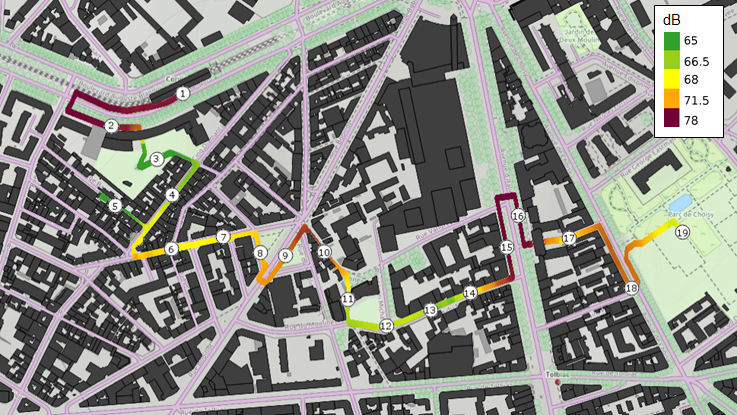
\includegraphics[width=.4\linewidth]{pictures/trajet_19pts.png}
\caption{Map of the soundwalk with the 19 stop points}
\end{figure}


\end{frame}

%%%%%%%%%%%%%%%%%%%%%%%%%%%%%%%%%%%%%%%%%%
%%%%%%%%%%%%%%%%%%%%%%%%%%%%%%%%%%%%%%%%%%

\begin{frame}{Study of urban sound recordings}
\begin{itemize}
	\item Annotation of each audio file 
	\begin{itemize}
		\item sound classes, begin and end times
	\end{itemize}
	

\end{itemize}

\begin{block}{From the observations and the annotations}
\begin{itemize}
	\item Synthesis of the 74 real scenes with \textit{simScene} with the \textit{replicate} mode
	\item 15 seconds example of a simulated scene\\
	
\centering
\includemedia[addresource=15sExample_22.mp3, 
flashvars={source=15sExample_22.mp3&autoPlay=true}]{\fbox{Play}}{APlayer.swf}
	
\end{itemize}
\end{block}
\vspace{0.5cm}
$\Rightarrow$ Are the simulated scenes realistic enough ? 

\end{frame}


%%%%%%%%%%%%%%%%%%%%%%%%%%%%%%%%%%%%%%%%%%
%%%%%%%%%%%%%%%%%%%%%%%%%%%%%%%%%%%%%%%%%%
\section{Design of the perceptual test}

\begin{frame}{Design of the perceptual test}

\begin{block}{Objective}
\begin{itemize}
	\item Evaluation of the realism of the simulated scene among real recordings by a panel of listeners
\end{itemize}
\end{block}

\begin{itemize}
	\item 40 audio tested
	\begin{itemize}
		\item 30 seconds duration
		\item Normalization to the same the sound level
		\item 20 audio files from the real recordings and the same 20 replicated
	\end{itemize}
	
	\item 50 participants \\	
	$\Rightarrow$ Each judge cannot evaluate all the scene
\end{itemize}

\begin{block}{Partially Balanced Incomplete Block Design}
\begin{itemize}
	\item 20 audio files listen by each judge 
	\item Design the order of listening for each judge with a fair statistical distribution
	\item Each judge listen a mix of 10 real and 10 replicated scenes
\end{itemize}

\end{block}

\end{frame}

%%%%%%%%%%%%%%%%%%%%%%%%%%%%%%%%%%%%%%%%%%
%%%%%%%%%%%%%%%%%%%%%%%%%%%%%%%%%%%%%%%%%%

\begin{frame}{Design of the perceptual test}
\begin{itemize}
	\item Web-page administered online on the 8 February 2017 and closed 12 days later
	\item For each scene listened
	\begin{itemize}
		\item answer to the question 'Is the scene you listen seems, to you, realistic ?'
		\item evaluation on a 7 points scale 
		\item possibility to re-listen the scene and to put a comment
	\end{itemize}
	\item The gender (H/F), the age and the experience in the listening of urban sound environments are then asked
\end{itemize}

\begin{block}{Constitution of the panel}
\begin{itemize}
	\item 18 females and 31 males (1 not documented)
	\item Average age : 36 ($\pm$ 12) years old
	\item 62 $\%$ of the participant declared having NO experience in the listening of urban sound mixtures
\end{itemize}
\end{block}

\end{frame}

%%%%%%%%%%%%%%%%%%%%%%%%%%%%%%%%%%%%%%%%%%
%%%%%%%%%%%%%%%%%%%%%%%%%%%%%%%%%%%%%%%%%%
\section{Results}
%\begin{frame}{Results}
%
%\begin{block}{ANalyse Of VAriance}
%\begin{itemize}
%	\item ANOVA to evaluate 
%	\item $H_0$ hypothesis : the distribution of note between the real and the simulated scenes cannot be discernible
%	\item $H_0$ hypothesis rejected if \textit{p-value} $< \alpha = 0.05$ 
%\end{itemize}
%\end{block}
%
%\end{frame}
%%%%%%%%%%%%%%%%%%%%%%%%%%%%%%%%%%%%%%%%%%
%%%%%%%%%%%%%%%%%%%%%%%%%%%%%%%%%%%%%%%%%%

\begin{frame}{Results}

\begin{block}{According to the 'type'}

\begin{figure}

\begin{flushleft}
\begin{minipage}[l]{.5\linewidth}
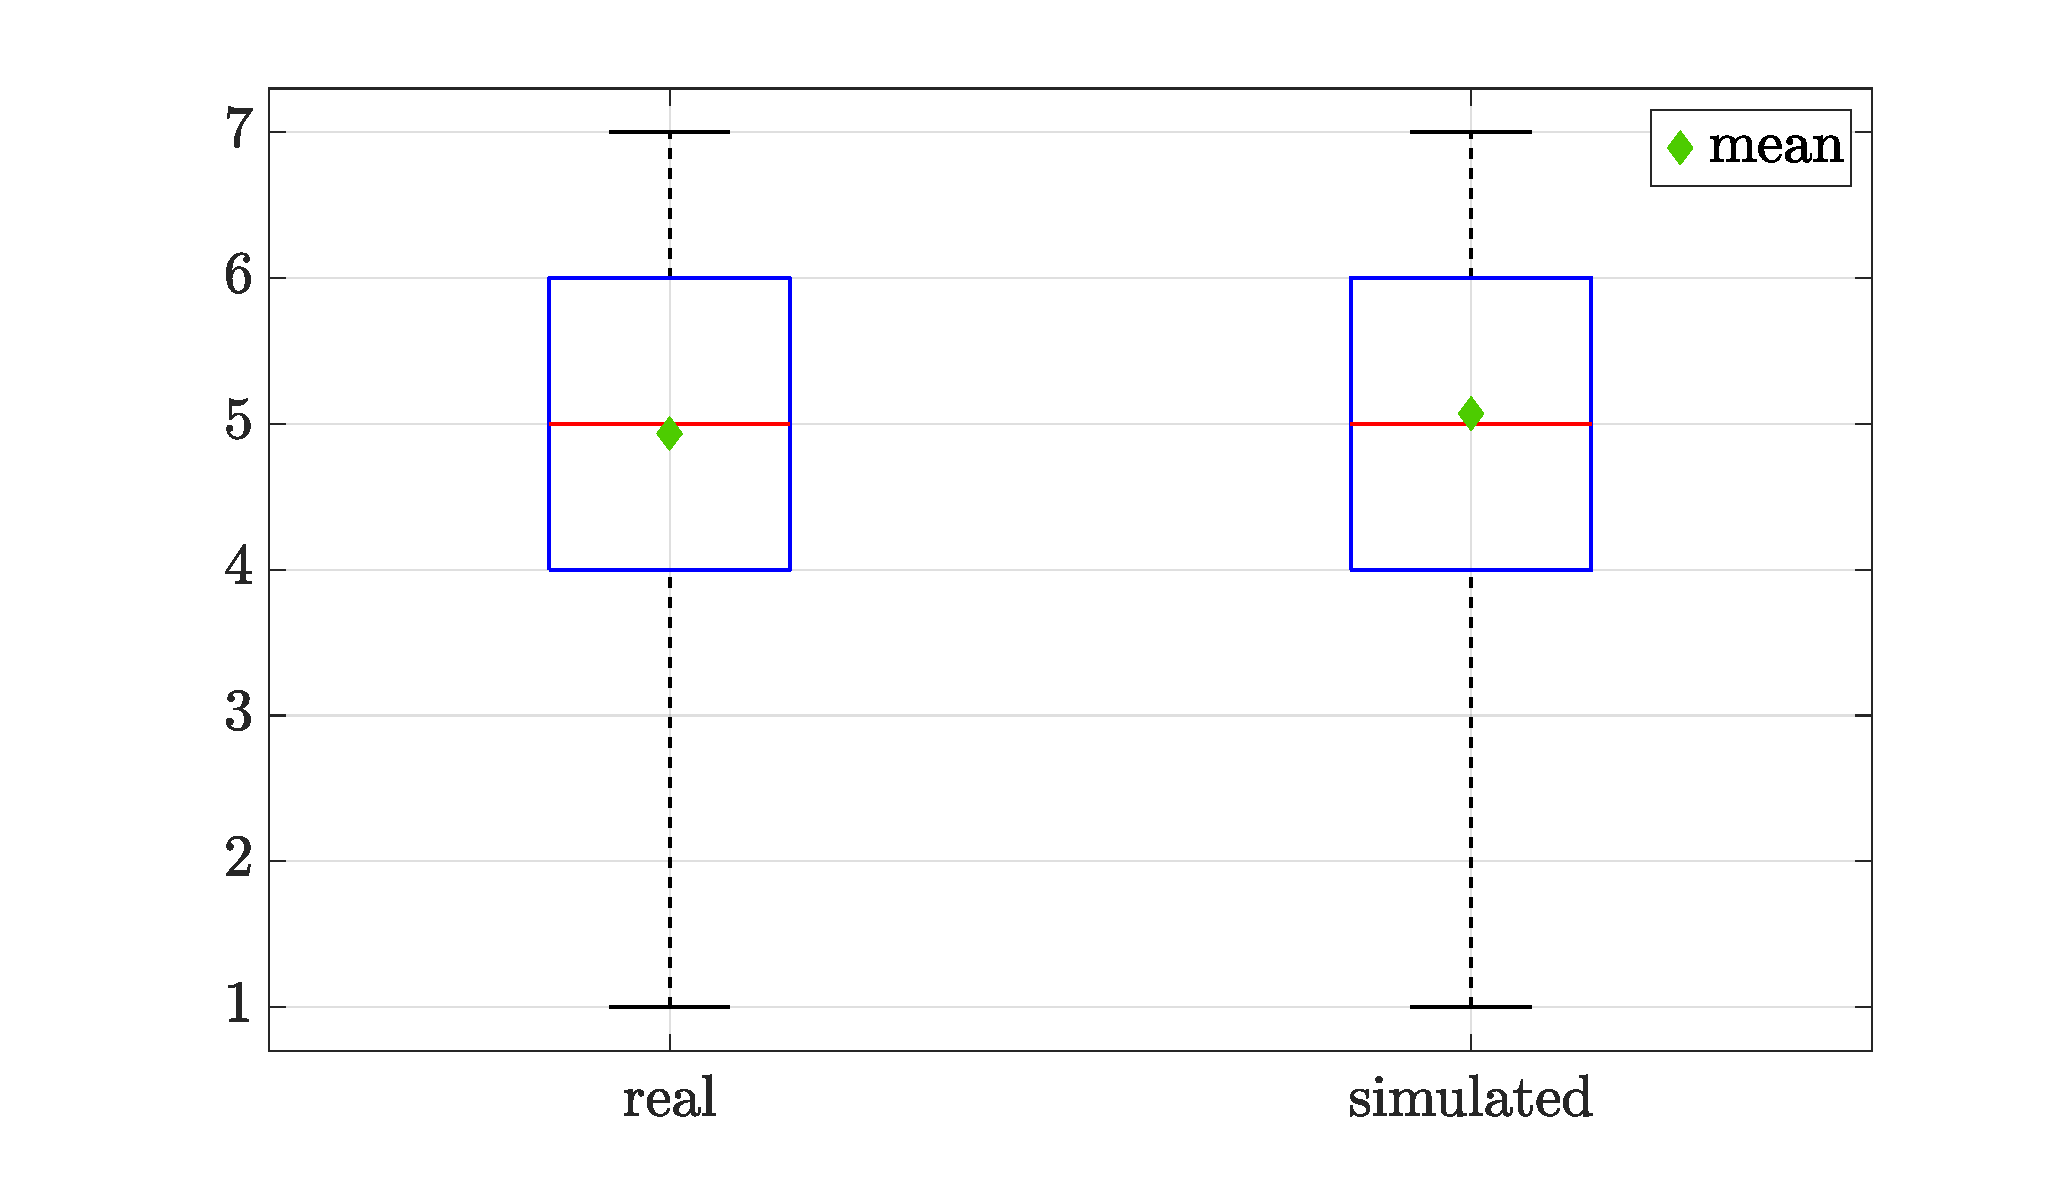
\includegraphics[width=\textwidth]{pictures/testPerceptif_boxplotType_EN.pdf}
\captionof{figure}{\footnotesize  Box-and-whiskers plot of the rating of realism according to the type of scene}
\end{minipage}
\hspace{0.1cm}
\begin{minipage}[r]{.4\linewidth}
\begin{itemize}
\footnotesize
	\item Hypothesis test $H_0$ : the distribution of the scores between the real and simulated scenes are similar
	\item Significance level $\alpha$ = 5 $\%$ to reject $H_0$
\end{itemize}

\footnotesize
\begin{tabular}{lccc}
	& DOF & $\vert t \vert$    & \textit{p-value} \\ 
\hline
type & 49 & 1.37 & 0.17    \\
\hline 
\end{tabular}
\captionof{table}{\footnotesize Paired sample \textit{t-test} }
\label{blablatab}
\end{minipage}

\end{flushleft}

\end{figure}
\end{block}

\begin{itemize}
\footnotesize
	\item T-test performed between the mean scores of the real and simulated scenes for each judge
	\item Real and simulated scenes evaluated in a similar way (\textit{p-value} $> \alpha = 0.05$)\\
\end{itemize}

$\Rightarrow$ Validation of the urban sound mixtures realism


\end{frame}

%%%%%%%%%%%%%%%%%%%%%%%%%%%%%%%%%%%%%%%%%%
%%%%%%%%%%%%%%%%%%%%%%%%%%%%%%%%%%%%%%%%%%


\begin{frame}{Results}

\begin{block}{According to the 'type', judge' and 'sound env.' factors}
\begin{figure}
\begin{flushleft}

\begin{minipage}[l]{.4\linewidth}		
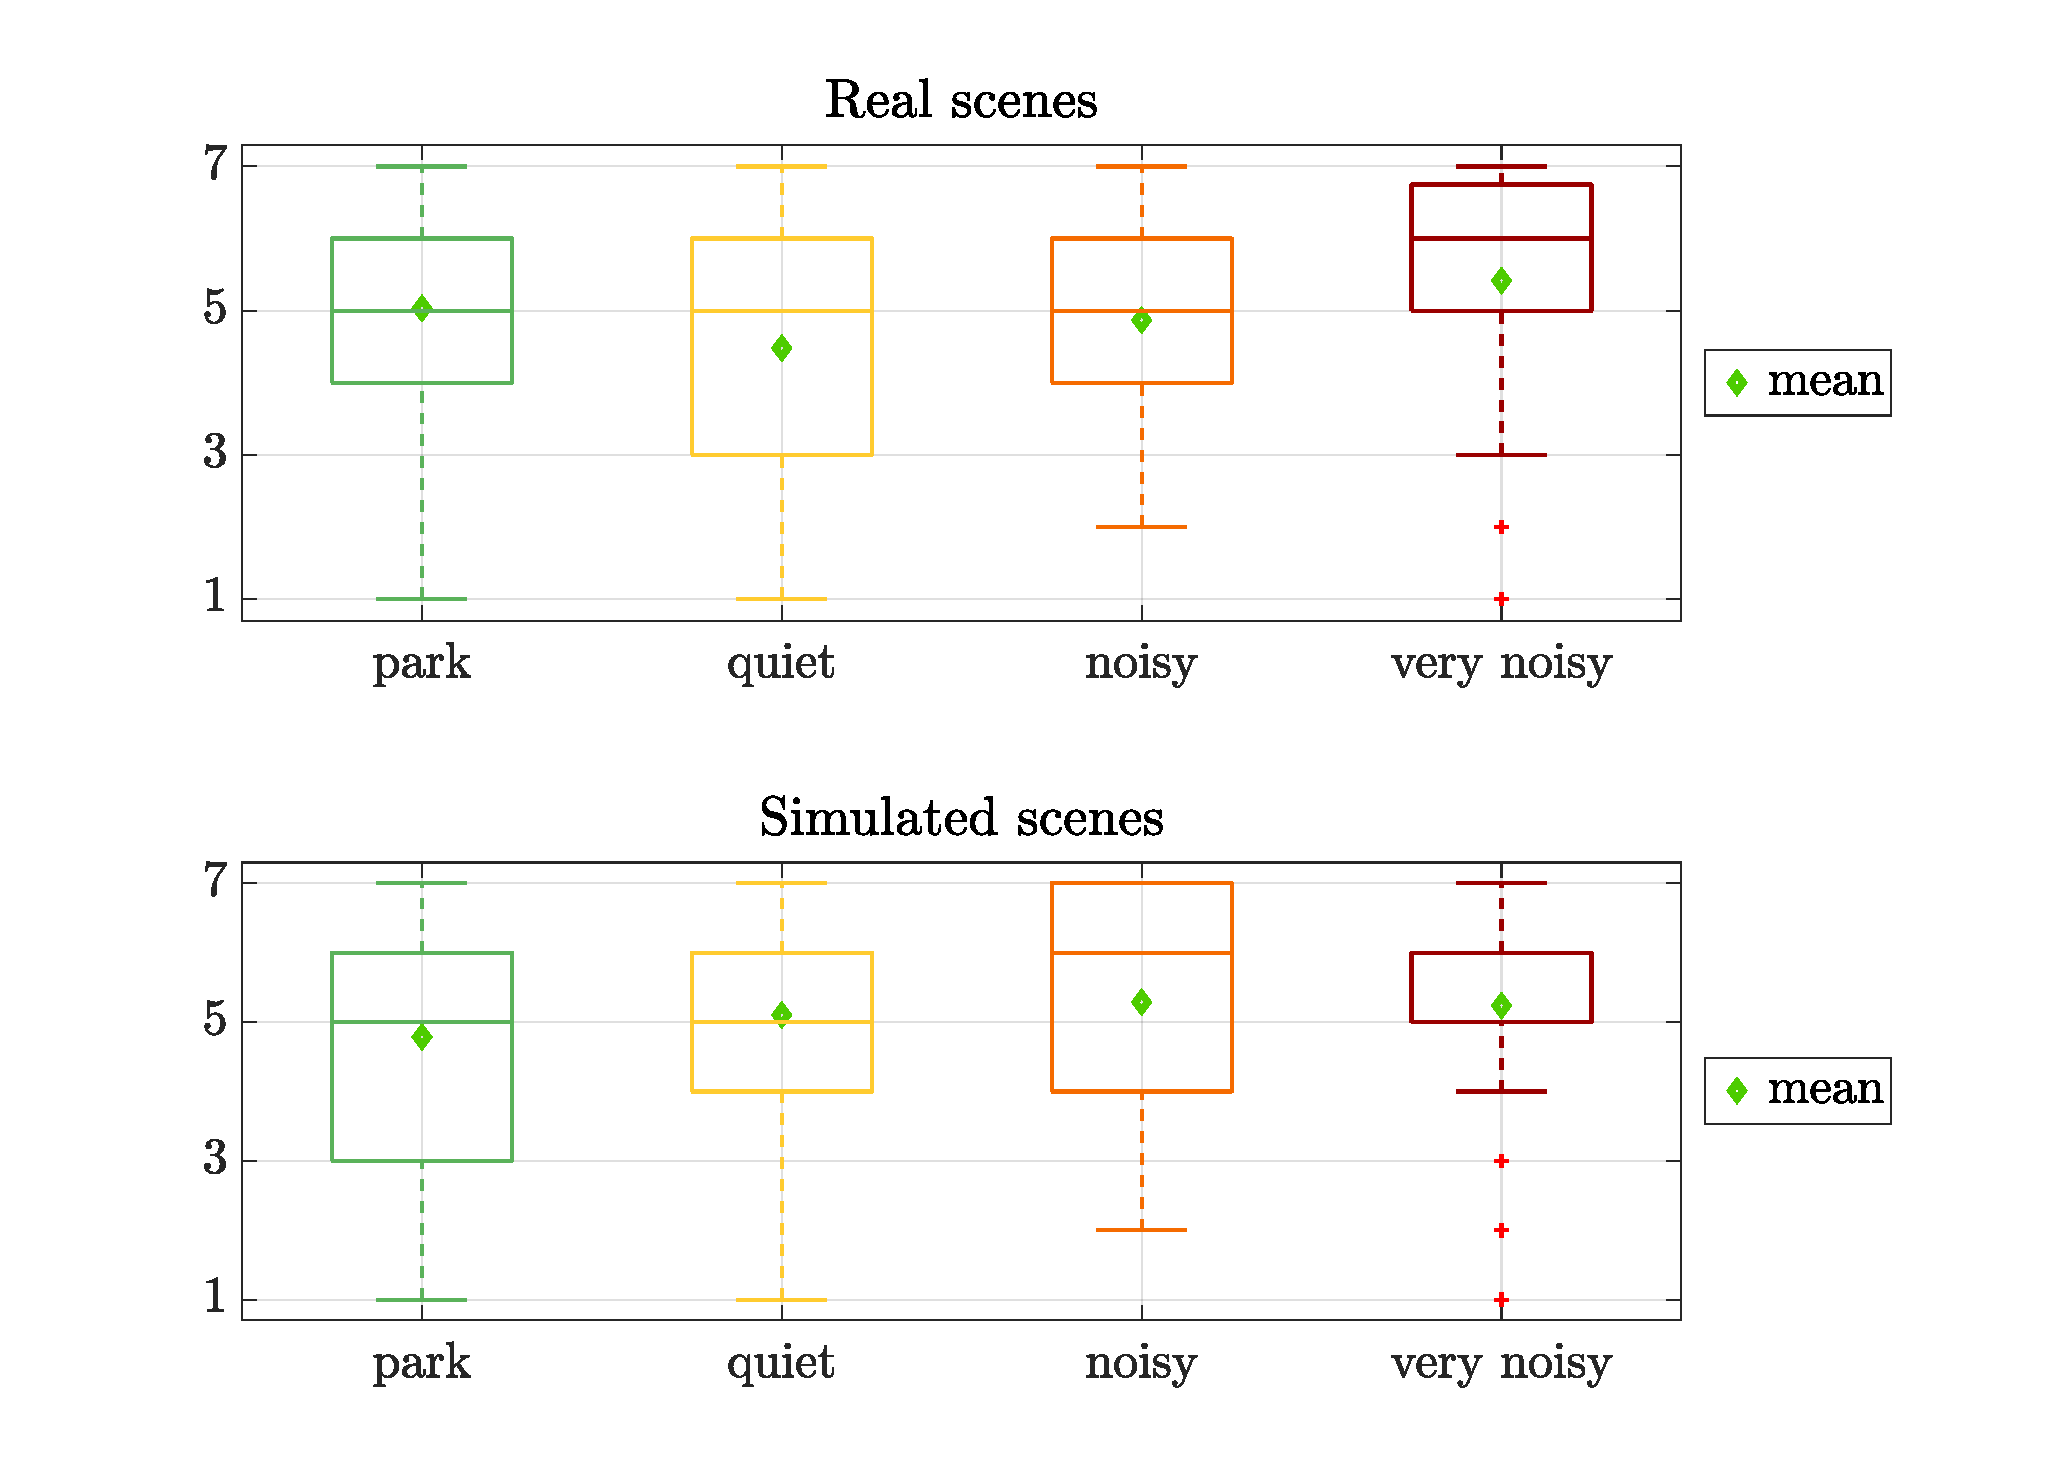
\includegraphics[width=\textwidth]{pictures/testPerceptif_boxplotAmbianceCOLOR_EN.pdf}
\captionof{figure}{\footnotesize Data distribution for the 'scene type' and 'sound environment' factors}
\end{minipage}% à retirer pour voir la différence.	
\begin{minipage}[r]{.5\linewidth}
\footnotesize
\begin{tabular}{p{2.35cm}p{0.5cm}p{0.95cm}p{1.65cm}}
        &  DOF &  \textit{F-stat.}    &  \textit{p-value} \\ 
\hline
 type &  1 &  1.38 &  0.24   \\
\hline
 sound env.   &  3 &  4.69 &  3.60$\times 10^{-3}$  \\ 
\hline
 judge   &  49 &  5.00 &  0.18$\times 10^{-9}$  \\ 
\hline
 type/sound env. &  3 &  6.80 &  0.20$\times 10^{-3}$\\
\hline
 type/judge &  49 &   1.07 &   0.35\\
\hline
 sound env./judge &  147 &  1.43 &  1.60$\times 10^{-3}$\\
\end{tabular}
\captionof{table}{\footnotesize Three-ways ANOVA}
\label{tab:p_value_type_ambience}
\end{minipage}
\end{flushleft}
\end{figure}
\end{block}


\begin{itemize}
\footnotesize
	\item Distribution between real and simulated scenes non significant again
	\item Interaction between sound env./judge and type/sound env.\\
	$\Rightarrow$ Evolution of the distributions different according to the levels
\end{itemize}

\end{frame}

%%%%%%%%%%%%%%%%%%%%%%%%%%%%%%%%%%%%%%%%%%
%%%%%%%%%%%%%%%%%%%%%%%%%%%%%%%%%%%%%%%%%%

\begin{frame}{Results}
\begin{block}{Interaction between the 'type' and 'sound environment' factors}
\begin{minipage}[l]{0.5\linewidth}		
\begin{figure}[hbtp]
\centering
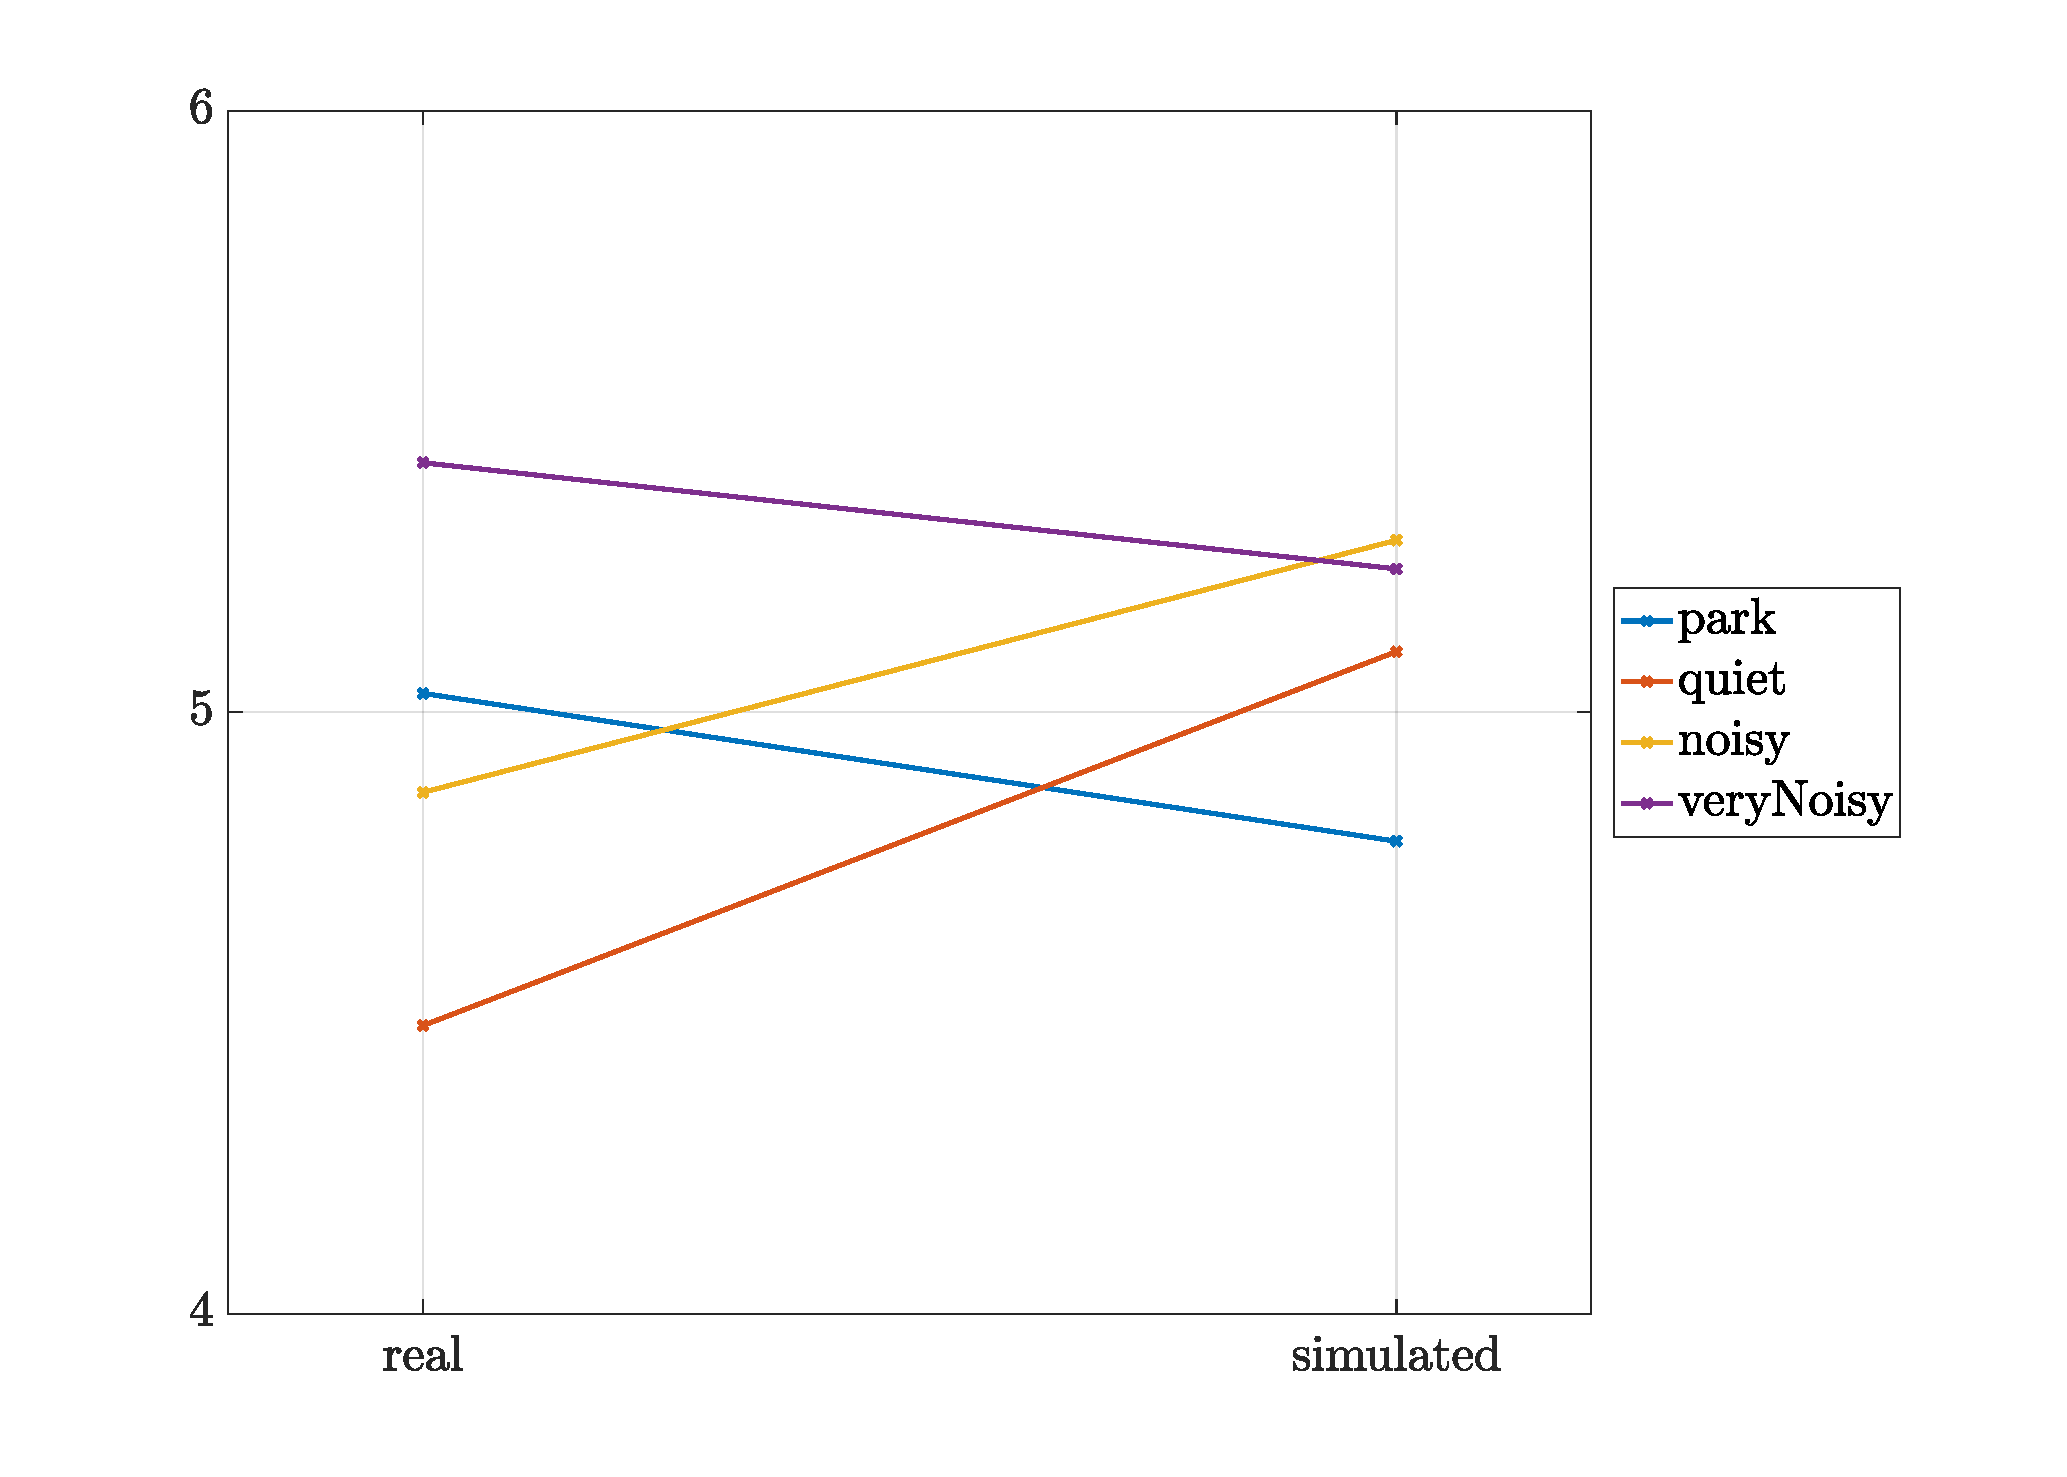
\includegraphics[width=\textwidth]{pictures/testPerceptif_interactionAmbianceCOLOR_EN.pdf}
\caption{Mean scores for the 4 sound environments according to the type}
\end{figure}
\end{minipage}% à retirer pour voir la différence.	
\begin{minipage}[c]{0.5\linewidth}
\begin{itemize}
\footnotesize
	\item We cannot conclude on the influence of the factors on the score
	\item Better mean scores for the 'noisy' and 'veryNoisy' simulated scenes
	\item Comments let by the panelists reveal that some noises are too loud (foot steps and birds) on the park and quiet simulated scenes
\end{itemize}

\end{minipage}
\end{block}

\end{frame}


%%%%%%%%%%%%%%%%%%%%%%%%%%%%%%%%%%%%%%%%%%
%%%%%%%%%%%%%%%%%%%%%%%%%%%%%%%%%%%%%%%%%%
\section{Conclusion}
\begin{frame}{Conclusion}

\begin{itemize}
\item Design of a corpus of realistic urban scenes 
\item Based on the annotation of 74 real recordings 
\item Use of the simulation software \textit{simScene}
\item Representative sound database of isolated sounds with car passages recorded specifically
\item The realism of the simulated scene is validated by a perceptual test
	\begin{itemize}
	\item No notable difference between the evaluation of the real and the simulated scenes
	\item The 'park' and 'quiet street' atmospheres are both perceived as less realistic than the 'noisy' and 'very noisy street' atmosphere
	\item some improvement can be made on the sound level of some sound classes (bird, foot step)
	\end{itemize}
\item Urban sound scene corpus that can be use to test sound recognition, classification or separation tools or to realize specific perceptual tests
\end{itemize}

\end{frame}

\begin{frame}

\titlepage

\end{frame}

\end{document}
